\section{Introdução}

Os sistemas reais nem sempre possuem o comportamento de saída como o desejado, seja pelas não idealidades dos componentes ou pela própria dinâmica do sistema. Considerando a impossibilidade de alterar essas particularidades, seja por os componentes não serem acessíveis à modificação ou se o acesso seja invasivo ao sistema, surge a necessidade de projetar controladores.

O controladores procuram avaliar as saídas atuais do sistema e, com base em certos parâmetros, atuar na entrada do sistema para que a saída se comporte como desejada. Não necessitando que altere a dinâmica do sistema original. 

Dessa forma, o presente trabalho tem o objetivo de projetar controladores por realimentação negativa e por realimentação de estados para a planta modelada pela função de transferência da equação \ref{planta:eq}. Os métodos de projeto de controladores PID por realimentação negativa (\textit{negative feedback}) compreendem: método pelo lugar das raízes, método polinomial e método frequencial. Já para o controlador por realimentação de estados (\textit{state feedback}) foi utilizado o método utilizando a fórmula de Ackermann

\begin{equation}\label{planta:eq}
    G_p(s) = \frac{2}{s(s+0,5)}
\end{equation}

Por meio do Scilab simula-se inicialmente o sistema em malha aberta e fechada sem o uso de controladores, de forma a avaliar se há a necessidade de projetar um controaldor.

Para simular o sistema em malha aberta, montou-se o diagrama mostrado na figura ~\ref{xcos:ma:a} e se obteve a saída conforme ilustra a figura ~\ref{xcos:ma:b}. Assim, percebe-se uma instabilidade no sistema, promovida pela presença do integrador na planta.

\begin{figure}[H]
\begin{center}
    \subfigure[Diagrama de blocos]{             
        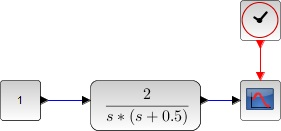
\includegraphics[width=5.5cm]{images/metodo_frequencial/xcosOL.jpg}  
        \label{xcos:ma:a}
    }
    \subfigure[Simulação temporal]{                                              
        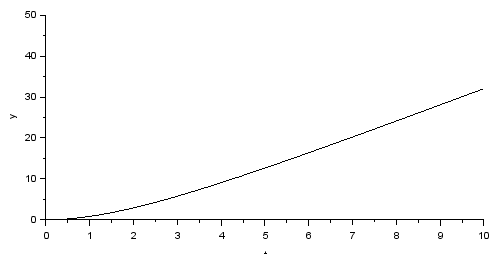
\includegraphics[width=9.5cm]{images/metodo_frequencial/timeOL.png}
        \label{xcos:ma:b}
    }                
\end{center}
\caption{Simulação com a planta em malha aberta no XCOS.}
\label{xcos:ma} 
\end{figure}

Colocando a planta em malha fechada, conforme mostra a figura ~\ref{xcos:mf:a}, obteve-se o desempenho expresso na figura ~\ref{xcos:mf:b}, apresentando um percentual de \textit{overshoot} de cerca de $57\%$ e tempo de estabilização de, aproximadamente, $14$ segundos. Assim, demonstrando a necessidade de um controle

\begin{figure}[H]
\begin{center}
    \subfigure[Diagrama de blocos]{             
        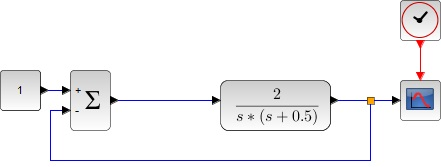
\includegraphics[width=6cm]{images/metodo_frequencial/xcosCL.jpg}  
        \label{xcos:mf:a}
    }
    \subfigure[Simulação temporal]{                                              
        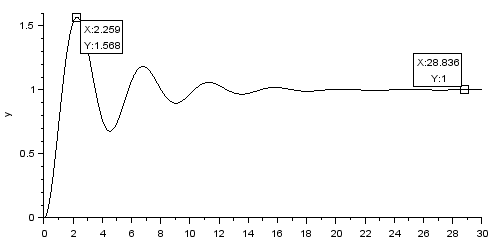
\includegraphics[width=9.5cm]{images/metodo_frequencial/timeCL.png}
        \label{xcos:mf:b}
    }                
\end{center}
\caption{Simulação com a planta em malha fechada no XCOS.}
\label{xcos:mf} 
\end{figure}
%\pagebreak